\documentclass[]{article}
\usepackage[left=1in,top=1in,right=1in,bottom=1in]{geometry}
\usepackage{graphicx}

%%%% more monte %%%%
% thispagestyle{empty}
% https://stackoverflow.com/questions/2166557/how-to-hide-the-page-number-in-latex-on-first-page-of-a-chapter
\usepackage{color}
% \usepackage[table]{xcolor} % are they using color?

% \definecolor{WSU.crimson}{HTML}{981e32}
% \definecolor{WSU.gray}{HTML}{5e6a71}

% \definecolor{shadecolor}{RGB}{248,248,248}
\definecolor{WSU.crimson}{RGB}{152,30,50} % use http://colors.mshaffer.com to convert from 981e32
\definecolor{WSU.gray}{RGB}{94,106,113}

%%%%%%%%%%%%%%%%%%%%%%%%%%%%

\newcommand*{\authorfont}{\fontfamily{phv}\selectfont}
\usepackage{lmodern}


  \usepackage[T1]{fontenc}
  \usepackage[utf8]{inputenc}




\usepackage{abstract}
\renewcommand{\abstractname}{}    % clear the title
\renewcommand{\absnamepos}{empty} % originally center

\renewenvironment{abstract}
 {{%
    \setlength{\leftmargin}{0mm}
    \setlength{\rightmargin}{\leftmargin}%
  }%
  \relax}
 {\endlist}

\makeatletter
\def\@maketitle{%
  \pagestyle{empty}
  \newpage
%  \null
%  \vskip 2em%
%  \begin{center}%
  \let \footnote \thanks
    {\fontsize{18}{20}\selectfont\raggedright  \setlength{\parindent}{0pt} \@title \par}%
}
%\fi
\makeatother









\title{\textbf{\textcolor{WSU.crimson}{Will vs
Denzel}} \newline \textbf{\textcolor{WSU.gray}{Who is better?}}  }
 

%  

% \author{ \Large true \hfill \normalsize \emph{} }
\author{\Large Minju
Lee\vspace{0.05in} \newline\normalsize\emph{Washington State
University}  }


\date{December 14, 2020}
\setcounter{secnumdepth}{3}

\usepackage{titlesec}
% See the link above: KOMA classes are not compatible with titlesec any more. Sorry.
% https://github.com/jbezos/titlesec/issues/11
\titleformat*{\section}{\bfseries}
\titleformat*{\subsection}{\bfseries\itshape}
\titleformat*{\subsubsection}{\itshape}
\titleformat*{\paragraph}{\itshape}
\titleformat*{\subparagraph}{\itshape}

% https://code.usgs.gov/usgs/norock/irvine_k/ip-092225/


%\titleformat*{\section}{\normalsize\bfseries}
%\titleformat*{\subsection}{\normalsize\itshape}
%\titleformat*{\subsubsection}{\normalsize\itshape}
%\titleformat*{\paragraph}{\normalsize\itshape}
%\titleformat*{\subparagraph}{\normalsize\itshape}

% https://tex.stackexchange.com/questions/233866/one-column-multicol-environment#233904
\usepackage{environ}
\NewEnviron{auxmulticols}[1]{%
  \ifnum#1<2\relax% Fewer than 2 columns
    %\vspace{-\baselineskip}% Possible vertical correction
    \BODY
  \else% More than 1 column
    \begin{multicols}{#1}
      \BODY
    \end{multicols}%
  \fi
}





\usepackage{natbib}
\setcitestyle{aysep={}} %% no year, comma just year
% \usepackage[numbers]{natbib}
\bibliographystyle{./../biblio/ormsv080.bst}



\usepackage[strings]{underscore} % protect underscores in most circumstances




\newtheorem{hypothesis}{Hypothesis}
\usepackage{setspace}


%%%%%%%%%%%%%%%%%%%%%%%%%%%%%%%%%%%%%%%%%%%%%%%%%%%%%
%%% MONTE ADDS %%%

\usepackage{fancyhdr} % fancy header 
\usepackage{lastpage} % last page 

\usepackage{multicol}


\usepackage{etoolbox}
\AtBeginEnvironment{quote}{\singlespacing\small}
% https://tex.stackexchange.com/questions/325695/how-to-style-blockquote


\usepackage{soul}			%% allows strike-through
\usepackage{url}			%% fixes underscores in urls
\usepackage{csquotes}		%% allows \textquote in references
\usepackage{rotating}		%% allows table and box rotation
\usepackage{caption}		%% customize caption information
\usepackage{booktabs}		%% enhance table/tabular environment
\usepackage{tabularx}		%% width attributes updates tabular
\usepackage{enumerate}		%% special item environment
\usepackage{enumitem}		%% special item environment

\usepackage{lineno}		%% allows linenumbers for editing using \linenumbers
\usepackage{hanging}


\usepackage{mathtools}  	%% also loads amsmath
\usepackage{bm}		%% bold-math
\usepackage{scalerel}	%% scale one element (make one beta bigger font)

\newcommand{\gFrac}[2]{ \genfrac{}{}{0pt}{1}{{#1}}{#2} }

\newcommand{\betaSH}[3]{  \gFrac{\text{\tiny #1}}{{\text{\tiny #2}}}\hat{\beta}_{\text{#3}}   }
\newcommand{\betaSB}[3]{              ^{\text{#1}} _{\text{#2}} \bm{\beta} _{\text{#3}}                   }  %% bold
\newcommand{\bigEQ}{  \scaleobj{1.5}{{\ }= } }
\newcommand{\bigP}[1]{  \scaleobj{1.5}{#1 } }





\usepackage{endnotes}  % he already does this ...
\renewcommand{\enotesize}{\normalsize}
% https://tex.stackexchange.com/questions/99984/endnotes-do-not-be-superscript-and-add-a-space
\renewcommand\makeenmark{\textsuperscript{[\theenmark]}} % in brackets %
% https://tex.stackexchange.com/questions/31574/how-to-control-the-indent-in-endnotes
\patchcmd{\enoteformat}{1.8em}{0pt}{}{}

\patchcmd{\theendnotes}
  {\makeatletter}
  {\makeatletter\renewcommand\makeenmark{\textbf{[\theenmark]} }}
  {}{}



% https://tex.stackexchange.com/questions/141906/configuring-footnote-position-and-spacing

\addtolength{\footnotesep}{5mm} % change to 1mm

\renewcommand{\thefootnote}{\textbf{\arabic{footnote}}}
\let\footnote=\endnote
%\renewcommand*{\theendnote}{\alph{endnote}}
%\renewcommand{\theendnote}{\textbf{\arabic{endnote}}}


\renewcommand*{\notesname}{}

\makeatletter
\def\enoteheading{\section*{\notesname
  \@mkboth{\MakeUppercase{\notesname}}{\MakeUppercase{\notesname}}}%
  \mbox{}\par\vskip-2.3\baselineskip\noindent\rule{.5\textwidth}{0.4pt}\par\vskip\baselineskip}
\makeatother


\renewcommand*{\contentsname}{TABLE OF CONTENTS}

\renewcommand*{\refname}{}


%\usepackage{subfigure}
\usepackage{subcaption}

\captionsetup{labelfont=bf}  % Make Table / Figure bold

%%% you could add elements here ... monte says .... %%%
%\usepackage{mypackageForCapitalH}


%%%%%%%%%%%%%%%%%%%%%%%%%%%%%%%%%%%%%%%%%%%%%%%%%%%%%

% set default figure placement to htbp
\makeatletter
\def\fps@figure{htbp}
\makeatother


% move the hyperref stuff down here, after header-includes, to allow for - \usepackage{hyperref}

\makeatletter
\@ifpackageloaded{hyperref}{}{%
\ifxetex
  \PassOptionsToPackage{hyphens}{url}\usepackage[setpagesize=false, % page size defined by xetex
              unicode=false, % unicode breaks when used with xetex
              xetex]{hyperref}
\else
  \PassOptionsToPackage{hyphens}{url}\usepackage[draft,unicode=true]{hyperref}
\fi
}

\@ifpackageloaded{color}{
    \PassOptionsToPackage{usenames,dvipsnames}{color}
}{%
    \usepackage[usenames,dvipsnames]{color}
}
\makeatother
\hypersetup{breaklinks=true,
            bookmarks=true,
            pdfauthor={Minju Lee (Washington State University)},
             pdfkeywords = {boxplots; descriptive statistics; pooled
t-test;},  
            pdftitle={Will vs Denzel: Who is better?},
            colorlinks=true,
            citecolor=blue,
            urlcolor=blue,
            linkcolor=magenta,
            pdfborder={0 0 0}}
\urlstyle{same}  % don't use monospace font for urls

% Add an option for endnotes. -----

%
% add tightlist ----------
\providecommand{\tightlist}{%
\setlength{\itemsep}{0pt}\setlength{\parskip}{0pt}}

% add some other packages ----------

% \usepackage{multicol}
% This should regulate where figures float
% See: https://tex.stackexchange.com/questions/2275/keeping-tables-figures-close-to-where-they-are-mentioned
\usepackage[section]{placeins}



\pagestyle{fancy}   
\lhead{\textcolor{WSU.crimson}{\textbf{ Will vs Denzel }}}
\chead{}
\rhead{\textcolor{WSU.gray}{\textbf{  Page\ \thepage\ of\ \protect\pageref{LastPage} }}}
\lfoot{}
\cfoot{}
\rfoot{}


\begin{document}
	
% \pagenumbering{arabic}% resets `page` counter to 1 
%    

% \maketitle

{% \usefont{T1}{pnc}{m}{n}
\setlength{\parindent}{0pt}
\thispagestyle{plain}
{\fontsize{18}{20}\selectfont\raggedright 
\maketitle  % title \par  

}

{
   \vskip 13.5pt\relax \normalsize\fontsize{11}{12} 
   
\textbf{\authorfont Minju Lee} \hskip 15pt \emph{\small Washington State
University}   

}

}








\begin{abstract}

    \hbox{\vrule height .2pt width 39.14pc}

    \vskip 8.5pt % \small 

\noindent The goal of this paper is to decide which actor is better
based on various metrics. The focus of the study is the popularity and
the monetary comparison between two actors. The methods I have used in
this study are descriptive statistics and inferential statistics. The
analysis shows a significant difference between the two actors.
\vspace{0.25in}

\noindent The paper explores the revenue and profit of the movies for
each actor domestically and internationally. It uses multiple boxplot
comparisons to give comprehensive visualization of monetary comparison
between the actors. Research moves onto popularity comparison, where
various metrics were compared in their mean values using inferential
statistics. \vspace{0.25in}

\noindent The analysis shows a significant difference between the two
actors' monetary comparison. However, popularity comparison could
improve its evaluation by possibly selecting more features from the IMDB
dataset.\vspace{0.25in}


\vskip 8.5pt \noindent \textbf{\underline{Keywords}:} boxplots;
descriptive statistics; pooled t-test; \par

    




    
    \hbox{\vrule height .2pt width 39.14pc}
    \vskip 5pt 
    \hfill \textbf{\textcolor{WSU.gray}{ December 14, 2020 } }
    \vskip 5pt 
    
\end{abstract}


\vskip -8.5pt



 % removetitleabstract

\noindent  

\section{Introduction}
\label{sec:intro}

\noindent  Will Smith was born on September 25th in 1968. He started his
acting career in 1990 in the TV series `The Fresh Prince of Bel-Air'. He
has gained success as a recording artist as well s a producer in films.
Denzel Washington was born on December of 28th in 1954. He first started
in the theater while working in the student drama production. His debut
was in the TV series called ``Carbon Copy'' in 1981. He works as an
actor, film producer, director, and also a screenwriter. Will Smith has
earned 4 Golden Globe Awards and 2 Academy Award nominations and several
Grammy Awards. On the other hand, Denzel Washinton has received 2 Golden
Globe Awards, 2 Academy Awards, and as well as a Tony
Award.\vspace{0.25in} \noindent  As we can see, they are both well-known
actors with many Awards. It is not so easy to distinguish who is better
than the other. Asking a question on who is a better actor is inherently
subjective, it is an arbitrary measure. There will be no right or wrong,
in the end, it is just an opinion. The goal of this paper is to come up
with the metrics to compare these actors objectively rather than
subjectively. The data was scraped from the IMDb website. The research
takes fish in the pond approach. It compares movies of each actor from
the popular 50 movies of each year from 1980 to 2019. Will was in 19
movies and Denzel was in 19 movies. There was a total of 1,998 movies in
this popular 50 movie list.In order to compare monetarily variables, I
have adjusted all the dollar values to the year 2000. \vspace{0.25in}

\begin{figure}[!ht]
    \hrule
    \caption{ \textbf{One Graphic: Will vs Denzel} }
    \begin{center}
        \scalebox{1.00}{    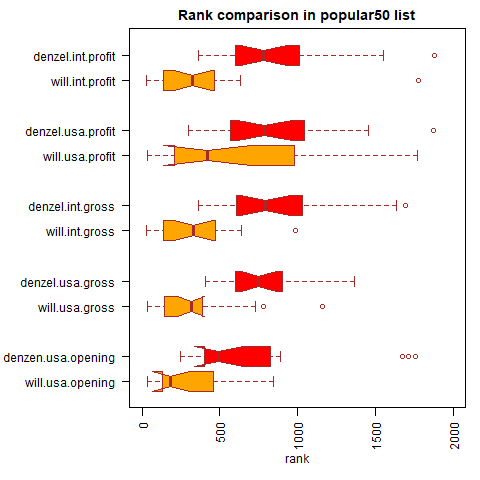
\includegraphics[trim = 0 0 0 0,clip,width=0.65\textwidth]{graphs/box_plot_comp.png} }
    \end{center}
    \label{fig:boxplot}
    \hrule
\end{figure}

\newpage

\noindent Figure \ref{fig:boxplot} The one graphic visualizes the
ranking distribution of each actor in the pond. The pond has 1,998
movies. Right off the bat, we can see both actors rank above average.
The average rank will be about 1000. These two actors are both popular
fish in the pond. We can also see that Will Smith outranks Denzel
Washington in every monetary metrics, this could be affected by many
things. Can genres of movies be correlated to revenue? Wills' majority
movie genres are comedy(41.4\%), drama(39.6\%), action(27.0\%), and
adventure(14.4\%). The majority of Denzels' movie genres are
drama(70.5\%), crime(34.4\%), action(29.5\%), and thriller(21.3\%).
According to the the-numbers.com(Statista,2020), adventure genre makes
the highest box office revenue in North America, followed by action,
drama, and comedy. \vspace{0.25in}

\section{Research Question:Monetary and popularity comparison between Will and Denzel}
\label{sec:rq}

\subsection{Who is better in terms of revenue/profit?}
\label{sec:rq2}

\noindent Figure \ref{fig:boxplot} shows Will dominates Denzel in
revenue and profit domestically and internationally. One interesting
thing to see is that despite Wills' clear dominance of U.S gross and U.S
profit distribution overlaps quite a bit. Wills' monetary success in
movies vary more in the U.S than internationally. Will might be popular
globally more than Denzel. The Table\ref{t.test} is a result of pooled
t-test on some of the variables between Will and Denzel. The null
hypothesis was set as Will smith has a higher mean than Denzel
Washington. The Variables of comparison were ratings, votes, budget,
profit in the U.S, and profit outside of the U.S. I have used a
significance level of 0.05. All of the results except the rating
variable shows the p-values smaller than 0.05. Thus, we cannot reject
our null hypothesis.\vspace{0.25in}

\subsection{Who is better in terms of popularity?}
\label{sec:rq2}

\noindent Popularity can be measured from the ratings, votes, and the
popular rank. The \ref{Table1} and \ref{Table2} shows summary statistics
of popularity for each of actors in popular 50 movies. Let's compare
average ratings, the average number of votes, and the average popular
rank. Denzel has an average rating of 7.3, an average number of 214792
votes, and an average popular rank of 24. Will has an average rating of
6.7, an average number of 335646 votes, and an average popular rank of
27. Will and Denzel both are at star-meter rank 500. However, will has
gone of 67, whereas Denzel has gone done 64 in his star-meter. Traffic
to the IMDB actor profile directly affects the star-meter of each
actor/actresses. Denzel has a better average rating about 9\% higher
than Will. Denzel also has a slightly high ranking than Will on the
popular movie list. However, Will receives about 120000 more votes on
average and had growing foot traffic to his actor page.\vspace{0.25in}

\subsection{Summary Statistics of Data}
\label{sec:data-summary}

% latex table generated in R 4.0.3 by xtable 1.8-4 package
% Mon Dec 14 22:37:24 2020
\begin{table}[ht]
\centering
\begin{tabular}{rrlrrrr}
  \hline
 & rank & title & year & ratings & votes & rank.popular \\ 
  \hline
&   1 & American Gangster & 2007 & 7.80 & 383980 &  15 \\ 
&   2 & Training Day & 2001 & 7.70 & 382022 &  15 \\ 
&   3 & Inside Man & 2006 & 7.60 & 332729 &  12 \\ 
&   4 & The Equalizer & 2014 & 7.20 & 326110 &   7 \\ 
&   5 & Man on Fire & 2004 & 7.70 & 324172 &  37 \\ 
&   6 & Flight & 2012 & 7.30 & 320297 &  27 \\ 
&   7 & Deja Vu & 2006 & 7.00 & 288953 &  17 \\ 
&   8 & The Book of Eli & 2010 & 6.90 & 288652 &  17 \\ 
&   9 & Philadelphia & 1993 & 7.70 & 219940 &  37 \\ 
&  11 & Remember the Titans & 2000 & 7.80 & 194611 &  11 \\ 
&  15 & The Magnificent Seven & 2016 & 6.90 & 181889 &  10 \\ 
&  17 & The Equalizer 2 & 2018 & 6.70 & 126514 &  28 \\ 
&  19 & Glory & 1989 & 7.80 & 119801 &   7 \\ 
&  21 & Crimson Tide & 1995 & 7.30 & 99414 &  47 \\ 
&  24 & Malcolm X & 1992 & 7.70 & 83628 &  18 \\ 
&  25 & The Pelican Brief & 1993 & 6.60 & 75635 &  39 \\ 
&  26 & Fallen & 1998 & 7.00 & 73486 &  48 \\ 
&  31 & Much Ado About Nothing & 1993 & 7.30 & 44429 &  36 \\ 
   \hline
\end{tabular}
\end{table}

% latex table generated in R 4.0.3 by xtable 1.8-4 package
% Mon Dec 14 22:41:11 2020
\begin{table}[ht]
\centering
\begin{tabular}{rrlrrrr}
  \hline
 & rank & title & year & ratings & votes & rank.popular \\ 
  \hline
&   1 & I Am Legend & 2007 & 7.20 & 675160 &  16 \\ 
&   2 & Suicide Squad & 2016 & 6.00 & 588064 &   4 \\ 
&   3 & Independence Day & 1996 & 7.00 & 520592 &  10 \\ 
&   4 & Men in Black & 1997 & 7.30 & 507597 &  19 \\ 
&   5 & I, Robot & 2004 & 7.10 & 491474 &  38 \\ 
&   6 & The Pursuit of Happyness & 2006 & 8.00 & 438121 &  27 \\ 
&   7 & Hancock & 2008 & 6.40 & 437887 &  39 \\ 
&   8 & Men in Black II & 2002 & 6.20 & 337458 &  36 \\ 
&   9 & Men in Black 3 & 2012 & 6.80 & 329948 &  48 \\ 
&  10 & Hitch & 2005 & 6.60 & 291991 &  35 \\ 
&  12 & Bad Boys & 1995 & 6.90 & 235766 &  12 \\ 
&  13 & Bad Boys II & 2003 & 6.60 & 228329 &  26 \\ 
&  14 & Enemy of the State & 1998 & 7.30 & 224019 &  32 \\ 
&  15 & Aladdin & 2019 & 7.00 & 216257 &  38 \\ 
&  16 & Austin Powers: The Spy Who Shagged Me & 1999 & 6.60 & 214064 &  27 \\ 
&  17 & Focus & 2015 & 6.60 & 212789 &  46 \\ 
&  23 & The Karate Kid & 2010 & 6.20 & 158842 &  10 \\ 
&  24 & Wild Wild West & 1999 & 5.00 & 151132 &  34 \\ 
&  25 & The Parent Trap & 1998 & 6.50 & 117780 &   8 \\ 
   \hline
\end{tabular}
\end{table}


\newpage

\subsection{Inferential analysis}
\label{sec:inference}

% latex table generated in R 4.0.3 by xtable 1.8-4 package
% Mon Dec 14 22:37:23 2020
\begin{table}[ht]
\centering
\hspace*{-3cm}
\begin{tabular}{rlllrrrrrlll}
  \hline
 & Variable & group1 & group2 & n1 & n2 & statistic & p & df & method & alternative & p.signif \\ 
  \hline
& ratings & Will Smith & Denzel Washigton &  19 &  18 & -3.66 & 0.00 & 31.05 & T-test & less & *** \\ 
& votes & Will Smith & Denzel Washigton &  19 &  18 & 2.59 & 0.01 & 32.68 & T-test & greater & ** \\ 
& budget.millions2000 & Will Smith & Denzel Washigton &  19 &  18 & 4.09 & 0.00 & 22.45 & T-test & greater & *** \\ 
& usa.profit.millions2000 & Will Smith & Denzel Washigton &  19 &  18 & 2.30 & 0.02 & 20.59 & T-test & greater & * \\ 
& international.profit.millions2000 & Will Smith & Denzel Washigton &  19 &  18 & 4.98 & 0.00 & 20.58 & T-test & greater & **** \\ 
   \hline
\end{tabular}
\caption{latex} 
\end{table}


\section{Key Findings}
\label{sec:findings}

\noindent Through analysis, some of the key differences were found. The
popular movies of Will Smith generated more cash on average than Denzel
Washington. Wills' Opening week revenues were about 209\% of Denzels'
opening week revenue, U.S gross was 193\% of Denzels' movies, world
gross was 253\% of Denzels' movies, international gross was 337\% of
Denzels' movies, U.S profit was 274\% of Denzels' movies, world profit
was 307\% of Denzels' movies, and international profit was 352\%
Denzels' movies. The popular movies of Wills' make about 2 to 3 times
more of Denzels`. Will smith particularly outperforms outside of the U.S
compared to Denzel.\vspace{0.25in}

\noindent Popularity comparison tells us that Denzel has about 9\%
higher ratings than Will. However, Will has about 56\% more votes than
Denzel. Also, the star-meter tells Denzel has been losing web traffic to
his actor page whereas Will has been gaining more web traffic to his
actor page.\vspace{0.25in}

\section{Conclusion}
\label{sec:conclusion}

\noindent After comparing all the metrics, I found out Will Smiths'
movies generate much more profits and the fact that he has a strong
international gross makes it hard to beat. Bringing money into the U.S
is even better for the economy than domestic transactions. Besides that,
Wills' movies make 2 to 3 times more revenue than Denzels. He is a clear
winner for the first battle. For popularity comparison, I have used
ratings, the number of votes, popular rank, and the star-meter. Here,
Denzel had better metrics on his ratings than Will. The pooled-t-test
result on rating metric tells us, indeed Wills' true average ratings
will be lower than Denzels'. However, Will's average number of votes
were significantly higher, and the pooled-t-test verifies that. Well, so
far they were tied. Therefore, I have decided to use the star-metric
delta values to decide the final winner for the popular comparison.
Looking at the star-metric delta value, Will has an increasing delta
value of 67 and Denzel has a decreasing delta value of 64. According to
the IMDB website, star-meters can tell you about public awareness and/or
interest in the actor. This could mean Will has high public influence
lately. Thus, I have chosen Will as the winner for the popularly
metric.\vspace{0.25in}

\noindent In conclusion, Will Smith scored higher on both monetary
metrics and popularity metrics. The metrics for popularity comparison
could improve on its feature selection. Unfortunately, Denzel has lost
this battle. Keep in mind, this does not represent beyond each actors'
monetary and popularity success. This does not mean Denzel is a bad
actor nor his movies terrible. I certainly don't judge one's ability to
act by their monetary success nor public popularity. Maybe, this could
be the next research question for continuing discussion. \vspace{0.25in}




%% appendices go here!


\newpage
\theendnotes

%%%%%%%%%%%%%%%%%%%%%%%%%%%%%%%%%%%  biblio %%%%%%%%
\newpage
\begin{auxmulticols}{2}
\singlespacing 
\bibliography{./../biblio/master.bib}

%%%%%%%%%%%%%%%%%%%%%%%%%%%%%%%%%%%  biblio %%%%%%%%
\end{auxmulticols}

\newpage
{
\hypersetup{linkcolor=black}
\setcounter{tocdepth}{3}
\tableofcontents
}



\end{document}